% Descripción de estos servidores 
Un servidor de impresión o servicio de impresión a gran escala es un servidor que conecta una impresora a una red para que cualquier PC pueda acceder a ella e imprimir trabajos, sin depender de otra PC para poder utilizarla.
\subsubsection{Instalación del servidor}
En esta sección se utilizó el servidor de impresiones CUPS (Common Unix Printing Server). Los pasos para su instalación son los siguientes:
\begin{figure}[!htbp]
	\hypertarget{fig:instalacionCUPS}{\hspace{1pt}}
	\begin{center}
		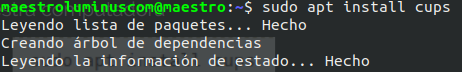
\includegraphics[width=0.7\textwidth]{desarrollo/tarea2/img/instalacionCUPS.png}
		\caption{Comando para instalar el servidor CUPS}
		\label{fig:instalacionCUPS}
	\end{center}
\end{figure}
\pagebreak
\begin{figure}[!htbp]
	\hypertarget{fig:respaldoCUPS}{\hspace{1pt}}
	\begin{center}
		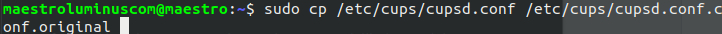
\includegraphics[width=0.7\textwidth]{desarrollo/tarea2/img/respaldoCUPS.png}
		\caption{Respaldamos la configuración original.}
		\label{fig:respaldoCUPS}
	\end{center}
\end{figure}
\pagebreak
\begin{figure}[!htbp]
	\hypertarget{fig:configCUPS}{\hspace{1pt}}
	\begin{center}
		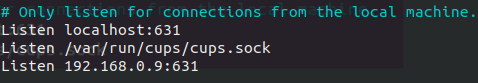
\includegraphics[width=0.7\textwidth]{desarrollo/tarea2/img/configCUPS.png}
		\caption{Agregamos otras direcciones que estará escuchando el servidor.}
		\label{fig:configCUPS}
	\end{center}
\end{figure}
\pagebreak
\begin{figure}[!htbp]
	\hypertarget{fig:reinicioCUPS}{\hspace{1pt}}
	\begin{center}
		
\includegraphics[width=0.7\textwidth]{desarrollo/tarea2/img/reinicioCUPS.png}
		\caption{Reiniciamos el servicio CUPS.}
		\label{fig:reinicioCUPS}
	\end{center}
\end{figure}